\documentclass[usenames,a4,landscape,semhelv]{seminar}
\usepackage{pst-all}
\usepackage{pst-blur}
\usepackage{rotate}
\usepackage{semcolor}
\usepackage{semlayer}
\input{seminar.bug}
\input{seminar.bg2}
\usepackage[activeacute,spanish]{babel}
\usepackage{amsbsy}
\usepackage{amssymb}
\usepackage{pifont}
\usepackage[ansinew]{inputenc}
\usepackage{pifont}
\usepackage{marvosym}
\usepackage[dvips]{graphicx}
\newcommand{\BibTeX}{\textsc{Bib}\textrm{\TeX}}
\newtheorem{theorem}{\color{blue}{Teorema}}[section]
%\newtheorem{acknowledgement}[theorem]{Acknowledgement}
\newtheorem{algorithm}[theorem]{Algoritmo}
\newtheorem{tarea}[theorem]{Tarea}
\newtheorem{axiom}[theorem]{Axioma}
\newtheorem{case}[theorem]{Caso}
\newtheorem{claim}[theorem]{Claim}
\newtheorem{conclusion}[theorem]{Conclusi\'on}
\newtheorem{conjecture}[theorem]{Conjetura}
\newtheorem{corollary}{Corolario}
\newtheorem{criterion}[theorem]{\color{blue}{Criterio}}
\newtheorem{definition}{\color{blue}{Definici\'on}}
\newtheorem{example}{\color{blue}{Ejemplo}}
\newtheorem{exercise}[theorem]{Ejercicios}
\newtheorem{lemma}{Lema}
\newtheorem{notation}[theorem]{Notaci\'on}
\newtheorem{problem}[theorem]{Problema}
\newtheorem{proposition}{Proposici\'on}
\newtheorem{remark}{\color{blue}{Observaci\'on}}
\newtheorem{solution}{\color{blue}{Soluci\'on}}[example]
\newtheorem{summary}[theorem]{Sumario}

%%%%%%%%%%%%%%%%%%%%%%%%%%%%%%%%%%%%%%%%%%%%%%%%%%%%%%%%%%%%%%%%%%%%%%%%%%
%%% directory from where eps-files are included
%%% list of directories like {{dir1}{dir2}...}

\graphicspath{{./}}

%%%%%%%%%%%%%%%%%%%%%%%%%%%%%%%%%%%%%%%%%%%%%%%%%%%%%%%%%%%%%%%%%%%%%%%%%%
%%% set some parameters

\def\initials{AO}
\def\name{Antalcides Olivo}
\def\place{Dpt de F�sica} % `place' or 'conference, place'
\def\month{07/2003} % format 'MM/YYYY'

%%%%%%%%%%%%%%%%%%%%%%%%%%%%%%%%%%%%%%%%%%%%%%%%%%%%%%%%%%%%%%%%%%%%%%%%%%
%%% page-style

\renewcommand{\slidetopmargin}{-0.2in}
\addtolength{\slidewidth}{1.5in} \extraslideheight{2mm}

\newcommand{\footcolor}{\Black}
\newcommand{\headtext}{}

\newsavebox{\myLoewe}
\sbox{\myLoewe}{
\includegraphics[scale=0.14]{logofoto.eps}}

\newpagestyle{mystyle}
{%
\rput[l]{0}(0,0)%
   {\psframebox[fillstyle=gradient,
                linecolor=White,
                gradmidpoint=0.45,
                gradlines=100,
                gradangle=90]
                {\begin{minipage}{0.98\textwidth}
                 {\large\bf \initials}
                 \quad
                 \rput{0}(0.2,0.11){\usebox{\myLoewe}}
                 \qquad\qquad
                 {\bf \place - \month}
                 \hfill\hfill\Red{\large\bf \headtext}
                 \end{minipage}}}
}% end header box
{%
\begin{minipage}{\textwidth}
\vspace*{-4truemm}
\hrulefill\\
\phantom{.}\hfill \footcolor{\name, \month}\hfill --\thepage--
\end{minipage}
}% end footer box

\slideframe{none}
\pagestyle{mystyle}


%%%%%%%%%%%%%%%%%%%%%%%%%%%%%%%%%%%%%%%%%%%%%%%%%%%%%%%%%%%%%%%%%%%%%%%%%%
%%% color-stuff

\definecolor{LightGray}{rgb}{0.94,0.94,0.94}
\definecolor{VeryLightBlue}{rgb}{0.9,0.9,1}
\definecolor{LightBlue}{rgb}{0.8,0.8,1}
\definecolor{DarkBlue}{rgb}{0,0,0.6}
\definecolor{LightGreen}{rgb}{0.88,1,0.88}
\definecolor{MidGreen}{rgb}{0.6,1,0.6}
\definecolor{DarkGreen}{rgb}{0,0.6,0}
\definecolor{VeryLightYellow}{rgb}{1,1,0.9}
\definecolor{LightYellow}{rgb}{1,1,0.6}
\definecolor{MidYellow}{rgb}{1,1,0.5}
\definecolor{VeryLightRed}{rgb}{1,0.9,0.9}
\definecolor{LightRed}{rgb}{1,0.8,0.8}

\newcommand{\VeryLightBlue}[1]{{\color{VeryLightBlue}{#1}}}
\newcommand{\LightBlue}[1]{{\color{LightBlue}{#1}}}
\newcommand{\Blue}[1]{{\color{Blue}{#1}}}
\newcommand{\DarkBlue}[1]{{\color{DarkBlue}{#1}}}
\newcommand{\DarkGreen}[1]{{\color{DarkGreen}{#1}}}
\newcommand{\VeryLightRed}[1]{{\color{VeryLightRed}{#1}}}
\newcommand{\LightRed}[1]{{\color{LightRed}{#1}}}
\newcommand{\Red}[1]{{\color{Red}{#1}}}
\newcommand{\Gray}[1]{{\color{Gray}{#1}}}
\newcommand{\Black}[1]{{\color{Black}{#1}}}

%%%%%%%%%%%%%%%%%%%%%%%%%%%%%%%%%%%%%%%%%%%%%%%%%%%%%%%%%%%%%%%%%%%%%%%%%%
%%% newcommands

\newcommand{\fnz}{\footnotesize}

%%%%%%%%%%%%%%%%%%%%%%%%%%%%%%%%%%%%%%%%%%%%%%%%%%%%%%%%%%%%%%%%%%%%%%%%%%
\begin{document}

% switch-on cumulative overlays
\makeatletter
\def\pst@initoverlay#1{%
\pst@Verb{%
/BeginOL {dup (all) eq exch TheOL le or {IfVisible not {Visible
/IfVisible true def} if} {IfVisible {Invisible /IfVisible false def} if}
ifelse} def
\tx@InitOL /TheOL (#1) def}}
\makeatother

% set some style parameters
\renewcommand{\headtext}{Universidad Del Norte}
\psset{gradbegin=MidYellow,gradend=MidGreen}
\renewcommand{\footcolor}{\DarkGreen}
%\psblurbox[fillstyle=solid,fillcolor=yellow,linecolor=red]

%%%%%%%%%%%%% slide 1 %%%%%%%%%%%%%
%\psblurbox[fillstyle=ccslope,linecolor=red,
%           slopebegin=MidYellow,slopeend=Red]
 \psblurbox[fillstyle=solid,fillcolor=yellow,linecolor=red]
{\begin{minipage}{0.5\textwidth}
  \vspace*{4mm}
 \Blue{\huge\bf F�sica calor}
 \vspace*{4mm}
  \end{minipage} }
  \vspace{6mm}
  \begin{center}\LARGE\bf
  Antalcides olivo\\
  Universidad del Norte\\
  e-mail: aolivo@uninorte.edu.co
\end{center}
  \vspace{0.5cm}
\sffamily {\small \noindent  \\ Copyright �{} 2003 Antalcides
Olivo Burgos. Universidad Del Norte}
%\begin{center}
\vspace*{6mm} \extraslideheight{1cm}
%{\begin{minipage}{0.5\textwidth}
%  \vspace*{4mm}
% \Blue{\huge\bf Estad\'{\i}stica}
% \vspace*{4mm}
%  \end{minipage} }
%  \vspace{6mm}
%  Antalcides olivo\\
%  Universidad del Norte\\
%  e-mail: aolivo@uninorte.edu.co\vspace{2.0cm}
%\sffamily {\small \noindent  \\ Copyright �{} 2003 Antalcides
%Olivo Burgos. Universidad Del Norte}
%\psblurbox[fillstyle=solid,fillcolor=yellow,linecolor=red]
%{\Blue{\huge\bf Repaso De Estad\'{\i}stica}} \vspace{4.8cm}
%\sffamily {\small \noindent  \\ Copyright �{} 2003 Antalcides
%Olivo Burgos. Universidad Del Norte}
%  e-mail: aolivo@uninorte.edu.co
%\begin{dinglist}{253}
%\overlay{1}{%
%\Blue{\item\Black{ {\Blue{\huge\bf �Qu\'{e} es la estad�stica?} }
\begin{slide}

\documentclass{article}
%%%%%%%%%%%%%%%%%%%%%%%%%%%%%%%%%%%%%%%%%%%%%%%%%%%%%%%%%%%%%%%%%%%%%%%%%%%%%%%%%%%%%%%%%%%%%%%%%%%%%%%%%%%%%%%%%%%%%%%%%%%%
%TCIDATA{OutputFilter=LATEX.DLL}
%TCIDATA{Created=Monday, September 29, 2003 10:29:43}
%TCIDATA{LastRevised=Monday, September 29, 2003 10:30:00}
%TCIDATA{<META NAME="GraphicsSave" CONTENT="32">}
%TCIDATA{<META NAME="DocumentShell" CONTENT="General\Blank Document">}
%TCIDATA{CSTFile=Math with theorems suppressed.cst}
%TCIDATA{PageSetup=72,72,72,72,0}
%TCIDATA{AllPages=
%F=36,\PARA{038<p type="texpara" tag="Body Text" >\hfill \thepage}
%}


\newtheorem{theorem}{Theorem}
\newtheorem{acknowledgement}[theorem]{Acknowledgement}
\newtheorem{algorithm}[theorem]{Algorithm}
\newtheorem{axiom}[theorem]{Axiom}
\newtheorem{case}[theorem]{Case}
\newtheorem{claim}[theorem]{Claim}
\newtheorem{conclusion}[theorem]{Conclusion}
\newtheorem{condition}[theorem]{Condition}
\newtheorem{conjecture}[theorem]{Conjecture}
\newtheorem{corollary}[theorem]{Corollary}
\newtheorem{criterion}[theorem]{Criterion}
\newtheorem{definition}[theorem]{Definition}
\newtheorem{example}[theorem]{Example}
\newtheorem{exercise}[theorem]{Exercise}
\newtheorem{lemma}[theorem]{Lemma}
\newtheorem{notation}[theorem]{Notation}
\newtheorem{problem}[theorem]{Problem}
\newtheorem{proposition}[theorem]{Proposition}
\newtheorem{remark}[theorem]{Remark}
\newtheorem{solution}[theorem]{Solution}
\newtheorem{summary}[theorem]{Summary}
\newenvironment{proof}[1][Proof]{\textbf{#1.} }{\ \rule{0.5em}{0.5em}}
\input{tcilatex}

\begin{document}


\end{document}

\end{slide}
%\begin{slide}
%\begin{center}
%
%%\rotatebox{90}{\resizebox{!}{2cm}{%
%%}
%%\vspace{6mm}
%%\begin{dinglist}{253}
%%\overlay{2}{%
%\Blue{\item\Black{ {\Blue{\huge\bf �Qu� es la estad�stica?}}%
%%% This document created by Scientific Word (R) Version 3.5

\documentclass{article}%
\usepackage{amsmath}%
\usepackage{amsfonts}%
\usepackage{amssymb}%
\usepackage{graphicx}
%TCIDATA{OutputFilter=latex2.dll}
%TCIDATA{LastRevised=Tuesday, July 22, 2003 14:31:06}
%TCIDATA{<META NAME="GraphicsSave" CONTENT="32">}
\section{Teor\'{\i}a de probabilidades}
\section{Experimentos y sucesos aleatorios}
\begin{definition}
Diremos que un experimento es aleatorio si se veri\-fican las siguientes condiciones,
\begin{enumerate}
\item Se puede repetir indefinidamente, siempre con las mismas condiciones.
\item Antes de realizarlo no se puede predecir el resultado.
\item El resultado ''$e"$ que se obtiene pertenece a un conjunto de resultados
posibles conocido previamente el cual llamaremos espacio muestral y lo
denotaremos con la letra $\Omega\;o\;S$. Los elementos del espacio muestral se
denominan sucesos elementales.
\end{enumerate}
\end{definition}
Es decir si $e_{1},e_{2}\in S\Longrightarrow e_{1},e_{2}$ son sucesos
elementales o puntos muestrales.En otras palabras: Un suceso es elemental si
su ocu\-rrencia o no ocurrencia no est\'{a} relacionada con ning\'{u}n otro suceso.
Cualquier subconjunto $A$ de $S$ se denomina suceso o evento aleatorio.
El espacio muestral puede ser de dos tipos:
\begin{itemize}
\item Discreto si est\'{a} formado por un conjunto finito o numerable de resultados.
\item Continuo si est\'{a} compuesto por un conjunto no numerable de elementos.
\end{itemize}
\begin{definition}
[Suceso determinista]Se denomina experimento determinista a el experimento que
al realizarlo varias veces con las mismas condiciones iniciales obtenemos
siempre el mismo resultado
\end{definition}
\begin{example}
Si dejamos caer dos cuerpos de diferentes masas y a la misma altura en el
vac\'{\i}o, los dos cuerpos caer\'{a}n al mismo tiempo.
\end{example}
Cuando en un experimento no se puede predecir el resultado final, decimos que
el experimento es aleatorio
\begin{example}
En una ruleta legal no se sabe que n\'{u}mero va a salir
\end{example}
\subsection{Probabilidad de laplace}
Si un experimento cualquiera se puede repetir obteniendo un n\'{u}mero finito
de resultados posibles y no existe ninguna raz\'{o}n para pensar que un
resultado tiene privilegios sobre otro, se calcula la probabi\-lidad del
suceso $A$ seg\'{u}n la regla de Laplace
\[
P\left(  A\right)  =\frac{n\acute{u}mero\,de\,casos\,favorables\,para\,A}{n\acute{u}mero\,de\,casos\,posibles}=\frac{n\left(  A\right)  }{n\left(
S\right)  }
\]
\begin{example}
Calcular la probabilidad de que al lanzar un dado se obtenga un n\'{u}mero par
\end{example}
\begin{solution}
El espacio muestral es $S=\{1,2,3,4,5,6\}$ llamaremos $A$ al suceso que da
como resultado un n\'{u}mero par el lanzamiento del dado, $A=\{2,4,6\},$ si
suponemos que el dado es legal, es decir ninguna cara tiene privilegio sobre
otra para salir, entonces
\[
P\left(  A\right)  =\frac{n\left(  A\right)  }{n\left(  S\right)  }=\frac
{3}{6}=\frac{1}{2}
\]
\end{solution}
\begin{definition}
\textbf{Definici\'{o}n axiom\'{a}tica de probabilidad}\newline Dado un espacio
muestral $S$, y una $\sigma-\acute{a}lgebra$ de sucesos $\mathcal{A}$ sobre
\'{e}l, diremos que $P$ es una probabilidad sobre $\mathcal{A}$ si cumple las
siguientes propiedades
\begin{description}
\item[A$_{1}$] La probabilidad es una funci\'{o}n definida sobre
$\ \mathcal{A}$, que toma solo valores positivos comprendidos entre 0 y 1, es
decir
\[
\begin{array}
[c]{ccc}
P:\mathcal{A} & \rightarrow & [0,1]\subset IR\\
A\in\mathcal{A} & \mapsto & 1\geq P\left(  A\right)  \geq0
\end{array}
\]
\item[A$_{2}$] La probabilidad del suceso seguro es 1
\[
P\left(  S\right)  =1
\]
\item[A$_{3}$] Para cualquier sucesi\'{o}n infinita $A_{1},A_{2},A_{3},\cdots$
de sucesos disjuntos de $\mathcal{A}$ se tiene que la probabilidad de el
evento $\bigcup_{i=1}^{\infty}A_{i}$ es la serie infinita de las
probabilidades, es decir
\end{description}
\end{definition}
\[
P\left(  \bigcup_{i=1}^{\infty}A_{i}\right)  =\sum_{i=1}^{\infty}P\left(
A_{i}\right)
\]
\subsubsection{propiedades}
$P\left(  \phi\right)  =0$
\begin{theorem}
Para cualquier sucesi\'{o}n finita de $n$ eventos disjuntos $A_{1},A_{2}
,A_{3},\cdots A_{n}\in\mathcal{A}$
\[
P\left(  \bigcup_{i=1}^{n}A_{i}\right)  =\sum_{i=1}^{n}P\left(  A_{i}\right)
\]
\end{theorem}
\begin{theorem}
para cualquier suceso $A\in\mathcal{A}$ se tiene que $P\left(  A^{\prime
}\right)  =1-P\left(  A\right)  $
\end{theorem}
\begin{theorem}
Si $A,B\in\mathcal{A}$ y $A\subset B$, entonces $P\left(  B\right)  \geq
P\left(  A\right)  $ y del A$_{1}$ $P\left(  B\cap A^{\prime}\right)  \geq0$
de lo que se deduce $P\left(  B\right)  \geq P\left(  A\right)  $
\end{theorem}
\begin{center}
\end{center}
\begin{theorem}
Para dos sucesos $A,B\subset\mathcal{A}$ cualesquiera $P\left(  A\cup
B\right)  =P\left(  A\right)  +P\left(  B\right)  -P\left(  A\cap B\right)  $
\end{theorem}
\begin{example}
Un estudiante de clase puede ser hombre o mujer. Si la probabilidad de que un
hombre sea seleccionado es 0.3 \textquestiondown Cu\'{a}l es la probabilidad
de que sea seleccionada una mujer?
\begin{solution}
Sea $A$ el evento de que se seleccione un hombre de la clase y sea $B$ el
evento de seleccionar una mujer, entonces es obvio que $S=A\cup B,$ y
adem\'{a}s $A\cap B=\phi,$ aplicando el teorema 7
\[
P\left(  A\cup B\right)  =P\left(  A\right)  +P\left(  B\right)  -P\left(
A\cap B\right)
\]
y de los teorema 4 y A$_{2}$ obtenemos
\begin{align*}
1  &  =P\left(  A\right)  +P\left(  B\right) \\
1  &  =0,3+P\left(  B\right) \\
P\left(  B\right)   &  =0,7
\end{align*}
\end{solution}
\end{example}
\begin{example}
Se selecciona una bola de una urna que contiene bolas rojas, blancas, azules,
amarillas y verdes. Si la probabilidad de seleccionar una bola roja es
$\frac{1}{5}$ y la de seleccionar una blanca es $\frac{2}{5}$
\textquestiondown Cu\'{a}l es la probabilidad de seleccionar una bola azul,
amarilla o blanca?
\end{example}
\begin{solution}
Sean $A_{1},A_{2},A_{3},A_{4},A_{5},A_{6}$ los eventos de seleccionar de la
urna una bola roja, blanca, azul, amarilla y verde respectivamente. Nos dicen
que $P\left(  A_{1}\right)  =$ $\frac{1}{5}$ y $P\left(  A_{2}\right)
=\frac{2}{5}$, entonces
\[
P\left(  A_{3}\cup A_{4}\cup A_{5}\cup A_{6}\right)  =P\left(  B\right)  =?
\]
Como los eventos son disjuntos
\[
S=A_{1}\cup A_{2}\cup A_{3}\cup A_{4}\cup A_{5}\cup A_{6}
\]
y por A$_{2}$ y el th.3
\begin{align*}
1  &  =P\left(  A_{1}\right)  +P\left(  A_{2}\right)  +P\left(  B\right) \\
P\left(  B\right)   &  =1-\frac{1}{5}-\frac{2}{5}=\frac{2}{5}
\end{align*}
\end{solution}
\begin{example}
Si la probabilidad de que un estudiante A pierda un examen de estad\'{\i}stica
es de 0,5, la probabilidad de que un estudiante B pierda el mismo examen es de
0,2 y la probabilidad de que ambos pierdan el examen es de 0,1
\end{example}
\begin{enumerate}
\item \textit{\textquestiondown Cu\'{a}l es la probabilidad de que al menos
uno de estos estudiantes gane el examen?}
\item \textit{\textquestiondown Cu\'{a}l es la probabilidad de de que ninguno
de los dos pierda el examen?}
\end{enumerate}
\begin{solution}
Sea $A$ el evento que el estudiante A pierda el examen y sea $B$ el evento de
que el estudiante B pierda el examen de estad\'{\i}stica
\end{solution}
\begin{description}
\item \textit{Nos piden la probabilidad de que uno de los dos gane el examen
pero no los dos, es decir si }$C$ \textit{es} \textit{este evento}
\begin{align*}
P\left(  C\right)   &  =P\left(  A^{\prime}\right)  +P\left(  B^{\prime
}\right)  -P\left(  A^{\prime}\cap B^{\prime}\right) \\
P\left(  A^{\prime}\right)   &  =1-P\left(  A\right)  =1-0,5=0,5\\
P\left(  B^{\prime}\right)   &  =1-P\left(  B\right)  =1-0,2=0,8\\
A^{\prime}\cap B^{\prime}  &  =\left(  A\cup B\right)  ^{\prime}\\
P\left(  A^{\prime}\cap B^{\prime}\right)   &  =1-P\left(  A\cup B\right)
\end{align*}
\textit{Pero}
\begin{align*}
P\left(  A\cup B\right)   &  =P\left(  A\right)  +P\left(  B\right)  -P\left(
A\cap B\right)  =0,6\\
P\left(  A^{\prime}\cap B^{\prime}\right)   &  =0,4
\end{align*}
\textit{entonces}
\[
P\left(  C\right)  =0,5+0,8-0,4=0,9
\]
\item $P\left(  A^{\prime}\cap B^{\prime}\right)  =0,4$
\end{description}
\section{T\'{e}cnica para la enumeraci\'{o}n de puntos muestrales}
Cuando $S$ o cualquiera de sus subconjuntos tiene muchos eventos elementales
describirlo por extensi\'{o}n para determinar los casos favorables y casos
posibles se hace engorroso por lo que en esta se\-cci\'{o}n utilizaremos el
an\'{a}lisis combinatorio para determinar los casos favorables y posibles de
una manera m\'{a}s simple.
\subsection{Diagrama de \'{a}rbol}
En experimentos simples es muy \'{u}til utilizar un m\'{e}todo llamado
diagrama de \'{a}rbol el cual explicar\'{e} con un ejemplo.
\begin{example}
Si se lanza una moneda legal tres veces \textquestiondown Cu\'{a}l es la
probabilidad de que \ en la primera y la ultima lanzada salga cara?.
%BeginExpansion
\begin{figure}
[ptb]
\begin{center}
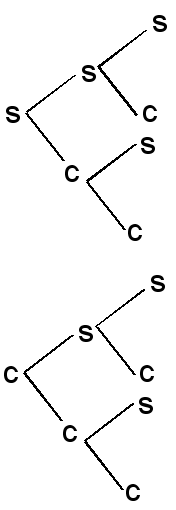
\includegraphics[
natheight=7.083700in,
natwidth=2.444800in,
height=2.7034in,
width=0.9504in
]{g11ir300.png}
\end{center}
\end{figure}
%EndExpansion
\end{example}
\begin{solution}
En el diagrama observamos que para el primer lanzamiento hay dos posibilidades
sello ($S$) y cara ($C$) en el segundo lanzamiento para cada posibilidad
anterior hay dos nuevas posibilidades y en el tercer se da lo mismo por lo que
al final hay 8 casos posibles y dos casos favorables de acuerdo con Laplace,
entonces si $A$ es el evento que sale cara en el primer y \'{u}ltimo
lanzamiento
\[
P\left(  A\right)  =\frac{2}{8}=\frac{1}{4}
\]
\end{solution}
\begin{theorem}
Consid\'{e}rese un experimento que tiene las dos cara\-cter\'{\i}sticas siguientes
\end{theorem}
\begin{itemize}
\item \textit{El experimento se realiza en dos partes }
\item \textit{La primera parte del experimento tiene }$m$ \textit{resultados
posibles }$x_{1},x_{2},x_{3},\cdots,x_{m}$ \textit{independientemente del
resultado} $x_{i}$ \textit{obtenido la segunda parte del experimento tiene
}$n$\textit{\ resultados posibles }$y_{1},y_{2},y_{3},\cdots,y_{n}
$\textit{.\newline Cada resultado del espacio muestral S del experimento
ser\'{a} por tanto, un par de la forma }$\left(  x_{i},y_{j}\right)
$\textit{\ es decir }
\begin{align*}
S  &  =\left\{  \left(  x_{i},y_{j}\right)  |i=1,2,3,\cdots m;j=1,2,3\cdots
n\right\} \\
n\left(  S\right)   &  =mn
\end{align*}
\end{itemize}
Este teorema puede generalizarse de la siguiente forma
Si un experimento \ puede realizarse con las siguientes caracter\'{\i}sticas
\begin{itemize}
\item El experimento se realiza en $k$ partes
\item la primera parte puede realizarse con $n_{1}$ resultados posibles
$x_{11},x_{12},x_{13},\cdots,x_{1n_{1}}$ e independientemente del resultado
$x_{1i}$ se pueden realizar la segunda parte con $n_{2}$ resultados posibles
$x_{21},x_{22},x_{23},\cdots,x_{2n_{2}}$ y as\'{\i} sucesivamente cada parte
del experimento puede realizarse de $n_{l}$ formas, $l=1,2,3,\cdots k$
obteni\'{e}ndose un espacio muestral de la forma
\begin{align*}
S  &  =\{(x_{1i},x_{2j},x_{3r},\cdots,x_{km})\}\\
n\left(  S\right)   &  =n_{1}\cdot n_{2}\cdot n_{3}\cdot\cdots\cdot n_{k}
\end{align*}
\end{itemize}
\section{Permutaciones}
\begin{definition}
Una permutaci\'{o}n es un arreglo de objetos distintos de tal manera que una
permutaci\'{o}n difiere de otra si el orden del arreglo o su contenido difieren
\end{definition}
Conviene observar que el orden es una caracter\'{\i}stica de especial
importancia en una permutaci\'{o}n. Cuando cambiamos el orden de los elementos
de este arreglo, se dice que permutamos dichos elementos
Consideremos un experimento en el cual se selecciona un objeto de $n$ objetos
distintos, y luego se selecciona un segundo objeto de los $n-1$ objetos
restantes, y as\'{\i} sucesivamente hasta seleccionar el \'{u}ltimo objeto
Este proceso \ se llama muestreo sin reemplazo\ de acuerdo con el teorema
anterior los $n$ objetos se pueden seleccionar de $n\left(  n-1\right)
\left(  n-2\right)  \cdots3\cdot2\cdot1$ $=n!$ formas diferentes\
Ahora si no se escogen todos los objetos, si no $k$ objetos, los $k$ objetos
se pueden seleccionar
\begin{align*}
p_{n,k}  &  =n\left(  n-1\right)  \left(  n-2\right)  \cdots\left(
n-k+1\right)  =\frac{n!}{\left(  n-k\right)  !}\;\;r\leq n\\
0!  &  =1\\
1!  &  =1\\
p_{n,n}  &  =n\left(  n-1\right)  \left(  n-2\right)  \cdots1=n!
\end{align*}
Supongamos que se necesitan dos representantes del grupo 02 de
estad\'{\i}stica I-ad para asistir a un congreso
\begin{solution}
Como el grupo 02 de estad\'{\i}stica tiene 40 alumnos y se necesitan dos, eso
quiere decir que que escogen 2 de 40
\[
p_{40,2}=\frac{40!}{\left(  40-2\right)  !}=1560
\]
\end{solution}
\begin{example}
Se necesita colocar 7 libros en un estante \textquestiondown De cuantas formas
posibles se pueden colocar?
\end{example}
\begin{solution}
Como se escoger\'{a}n 7 de 7 entonces
\[
p_{7,7}=7!=5040
\]
\end{solution}
Una combinaci\'{o}n es un arreglo de objetos distintos donde una
combinaci\'{o}n difiere de otra si difiere el contenido del arreglo. Si nos
interesa determinar el n\'{u}mero de combinaciones cuando en $n$ objetos
distintos deben seleccionarse $r$ a la vez entonces
\[
C_{n,r}=\frac{p_{n,r}}{r!}=\left(
\begin{array}
[c]{c}
n\\
r
\end{array}
\right)  \;\;r\leq n
\]
ya que el numerador es el n\'{u}mero de permutaciones al escoger $r$ objetos
de $n$ posibles, pero hay que descontar los casos en que el orden determina
para la combinaci\'{o}n el mismo elemento, que es exactamente $r!.$
\begin{example}
Una moneda se tira 10 veces.\ Calcular la probabi\-lidad de que aparezcan
exactamente 7 caras
\end{example}
\begin{solution}
Ya que la moneda tiene dos formas diferentes de aparecer en cada tiro, en 10
ser\'{\i}a $2^{10}$ formas. Y de las 10 caras vamos a seleccionar 7 caras, por
lo que ser\'{\i}an $C_{10,7}$ formas diferentes, por lo que la probabilidad
buscada es
\[
P=\frac{\binom{10}{7}}{2^{10}}=\frac{15}{128}
\]
\end{solution}
\begin{example}
Si se sacan $3$ cartas al azar de una baraja de $52$ cartas, calcular la
probabilidad de que sean as, rey y reina.
\end{example}
\begin{solution}
Se pueden seleccionar $3$ cartas al azar entre $52$, por lo que hay
$C_{52,3}\;$formas diferentes. Y como hay $4$palos y en cada palo hay un as,
un rey y una reina, entonces resulta que estas barajas pueden obtenerse de
$4\times4\times4$ formas diferentes .Por lo que la probabilidad buscada es
\[
\frac{4^{3}}{\binom{52}{3}}=\frac{16}{5525}=2.\,\allowbreak895\,9\times
10^{-3}
\]
\end{solution}
\begin{example}
De una bolsa que que contiene 4 bolas blancas, 2 negras y 3 rojas, se sacan 5
al azar. Calcular la probabilidad de que 2 sean blancas 1 negra y 2 rojas.
\end{example}
\begin{solution}
Del total de $4+2+3=9$ bolas se pueden seleccionar 5 bolas en $C_{9,5}$ formas
diferentes. Ahora entre las 4 bolas blancas 2 de ellas pueden seleccionarse
$C_{4,2}$, entre las 2 blancas $C_{2,1}$ y entre las 3 rojas $C_{3,2}$ formas
por lo que el total de casos favorables es $C_{4,2}C_{2,1}C_{3,2}$, as\'{\i}
\[
P=\frac{\binom{4}{2}\binom{2}{1}\binom{3}{2}}{\binom{9}{5}}=\frac{2}{7}
\]
\end{solution}
\section{Probabilidad condicionada e independencia de eventos}
\begin{definition}
Sean $A,B\in\mathcal{A}$ y sea $B$ un evento de probabilidad no nula para el
evento $A$, llamamos probabilidad condicionada de $A$ a $B$ a la cantidad que
representamos $P\left(  A|B\right)  $ y que definimos
\[
P\left(  A|B\right)  =\frac{P\left(  AB\right)  }{P\left(  B\right)  },
\]
la cantidad $P\left(  A|B\right)  $ se lee la probabilidad de $A$ dada la
ocu\-rrencia de $B$
\end{definition}
\begin{example}
Se lanza al aire un dado \textquestiondown Cu\'{a}l es la probabilidad de que
salga el n\'{u}mero 4? si sabemos que el resultado ha sido par
\end{example}
\begin{solution}
Sea $A=\{4\}$, entonces $P\left(  A\right)  =\frac{1}{6},$\newline
$B=\{2,4,6\},$ \ entonces $P\left(  B\right)  =\frac{3}{6}=\frac{1}{2}
$\newline por tanto
\[
P\left(  A|B\right)  =\frac{P\left(  AB\right)  }{P\left(  B\right)  }
=\frac{\frac{1}{6}}{\frac{1}{2}}=\frac{1}{3}
\]
\end{solution}
\begin{definition}
Sean $A,B\in\mathcal{A}$ dos eventos de probabilidad no nula se dice que son
independientes si y solo si
\[
P\left(  AB\right)  =P\left(  A\right)  P\left(  B\right)
\]
\end{definition}
\begin{example}
Para cierta poblaci\'{o}n de empleados, los porcentajes de quienes aprueban un
examen de aptitud para un trabajo, especificados seg\'{u}n el sexo, se
muestran en la tabla. Es decir todas las personas que presentan el examen el
24\% cae en la categor\'{\i}a de hombre aprobado, el 16\% en la categor\'{\i}a
de de hombre reprobado, y as\'{\i} sucesivamente. Se selecciona al azar un
empleado de esta poblaci\'{o}n. Sea $A$ el evento de que el empleado aprueba
el examen y $H$ el evento de que se selecciona un hombre \textquestiondown Son
independientes los eventos $A$ y $H$ ?
\[
\begin{tabular}
[c]{|c|c|}\hline
& sexo\\\hline
\begin{tabular}
[c]{l}
Resultado\\
Aprueba $\left(  A\right)  $\\
Reprueba$\left(  A^{\prime}\right)  $\\
Total
\end{tabular}
&
\begin{tabular}
[c]{lll}
Mujer$\left(  M\right)  $ & Hombre$\left(  H\right)  $ & Total\\
24 & 36 & 60\\
16 & 24 & 40\\
40 & 60 & 100
\end{tabular}
\\\hline
\end{tabular}
\]
\begin{solution}
Determinemos
\begin{align*}
P\left(  A|H\right)   &  =\frac{{}}{{}}\\
&  =\_\_\_\_\_\_\\
&  =\_\_\_\_\_\_\\
&  =\_\_\_\_\_\_\_
\end{align*}
\end{solution}
\end{example}
\begin{theorem}
(Bayes) Sea $A_{1},A_{2},A_{3},\cdots A_{n}\in\mathcal{A}$ un sistema
exhaustivo y excluyente de eventos. Sea $B\subset\mathcal{A}$ un suceso del
que conocemos todas las cantidades
\[
P\left(  B|A_{i}\right)  ,i=1,2,3,\cdots,n
\]
a las que denominamos verosimilitudes, entones se verifica
\[
\forall j=1,2,3,\cdots,n,\qquad P\left(  A_{j}|B\right)  =\frac{P\left(
B|A_{j}\right)  P\left(  A_{j}\right)  }{\sum_{i=1}^{n}P\left(  B|A_{i}\right)  P\left(  A_{i}\right)  }
\]
\end{theorem}
\begin{example}
Se tienen tres urnas. Cada una de ellas contiene un n\'{u}mero diferente de
bolas blancas y rojas. La primera urna tiene 3 bolas blancas y 2 rojas, la
segunda 4 bolas blancas y 2 rojas y la tercera 3 bolas rojas.\newline Se
realiza el siguiente experimento:\newline Algui\'{e}n elije al azar y con la
misma probabilidad una de las tres urnas, saca una bola.\newline Si el
resultado del experimento ha sido sacar una bola blanca
\textquestiondown \ Cu\'{a}l es la probabilidad de que provenga de la primera
urna? Calcular lo mismo para las otras dos urnas.
\end{example}
\begin{solution}
Si $B$: es el evento de sacar una bola blanca y $R$: el evento de sacar una
bola roja, entonces como \newline
\begin{tabular}
[c]{ll}
$U_{1}:$ & 3 bolas blancas y 2 rojas\\
$U_{2}:$ & 4 bolas blancas y 2 rojas\\
$U_{3}:$ & 3 bolas rojas
\end{tabular}
\newline tenemos
\begin{align*}
P\left(  U_{1}\right)   &  =\frac{1}{3}\\
P\left(  U_{2}\right)   &  =\frac{1}{3}\\
P\left(  U_{3}\right)   &  =\frac{1}{3}\\
P\left(  B|U_{1}\right)   &  =\frac{3}{5}\\
P\left(  B|U_{2}\right)   &  =\frac{4}{6}\\
P\left(  B|U_{3}\right)   &  =0
\end{align*}
En este caso $U_{1},U_{2},U_{3}$ forman un sistema incompatible y excluyente
de eventos, por lo que es posible aplicar el teorema de Bayes
\begin{align*}
P\left(  U_{1}|B\right)   &  =\frac{P\left(  B|U_{1}\right)  P\left(
U_{1}\right)  }{P\left(  B|U_{1}\right)  P\left(  U_{1}\right)  +P\left(
B|U_{2}\right)  P\left(  U_{2}\right)  +P\left(  B|U_{3}\right)  P\left(
U_{3}\right)  }\\
&  =\frac{\left(  \frac{3}{5}\right)  \left(  \frac{1}{3}\right)  }{\left(
\frac{3}{5}\right)  \left(  \frac{1}{3}\right)  +\left(  \frac{4}{6}\right)
\left(  \frac{1}{3}\right)  +0\left(  \frac{1}{3}\right)  }\\
&  =\frac{9}{19}
\end{align*}
\newline Para los otros dos casos resulta de manera equivalente
\begin{align*}
P\left(  U_{2}|B\right)   &  =\frac{P\left(  B|U_{2}\right)  P\left(
U_{2}\right)  }{P\left(  B|U_{1}\right)  P\left(  U_{1}\right)  +P\left(
B|U_{2}\right)  P\left(  U_{2}\right)  +P\left(  B|U_{3}\right)  P\left(
U_{3}\right)  }\\
&  =\frac{10}{19}
\end{align*}
\begin{align*}
P\left(  U_{3}|B\right)   &  =\frac{P\left(  B|U_{3}\right)  P\left(
U_{3}\right)  }{P\left(  B|U_{1}\right)  P\left(  U_{1}\right)  +P\left(
B|U_{2}\right)  P\left(  U_{2}\right)  +P\left(  B|U_{3}\right)  P\left(
U_{3}\right)  }\\
&  =0
\end{align*}
\end{solution}


\begin{document}

%%% This document created by Scientific Word (R) Version 3.5
%\documentclass{article}%
%\usepackage{amsmath}
%\usepackage{amsfonts}
%\usepackage{amssymb}
%\usepackage{graphicx}%
%\setcounter{MaxMatrixCols}{30}
%%TCIDATA{OutputFilter=latex2.dll}
%%TCIDATA{Version=4.00.0.2312}
%%TCIDATA{CSTFile=LaTeX article (bright).cst}
%%TCIDATA{Created=Friday, July 18, 2003 13:54:02}
%%TCIDATA{LastRevised=Sunday, July 20, 2003 14:51:02}
%%TCIDATA{<META NAME="GraphicsSave" CONTENT="32">}
%%TCIDATA{<META NAME="DocumentShell" CONTENT="Articles\SW\Standard LaTeX Article">}
%\newtheorem{theorem}{Theorem}
%\newtheorem{acknowledgement}[theorem]{Acknowledgement}
%\newtheorem{algorithm}[theorem]{Algorithm}
%\newtheorem{axiom}[theorem]{Axiom}
%\newtheorem{case}[theorem]{Case}
%\newtheorem{claim}[theorem]{Claim}
%\newtheorem{conclusion}[theorem]{Conclusion}
%\newtheorem{condition}[theorem]{Condition}
%\newtheorem{conjecture}[theorem]{Conjecture}
%\newtheorem{corollary}[theorem]{Corollary}
%\newtheorem{criterion}[theorem]{Criterion}
%\newtheorem{definition}[theorem]{Definition}
%\newtheorem{example}[theorem]{Example}
%\newtheorem{exercise}[theorem]{Exercise}
%\newtheorem{lemma}[theorem]{Lemma}
%\newtheorem{notation}[theorem]{Notation}
%\newtheorem{problem}[theorem]{Problem}
%\newtheorem{proposition}[theorem]{Proposition}
%\newtheorem{remark}[theorem]{Remark}
%\newtheorem{solution}[theorem]{Solution}
%\newtheorem{summary}[theorem]{Summary}
%\newenvironment{proof}[1][Proof]{\textbf{#1.} }{\ \rule{0.5em}{0.5em}}
%\begin{document}
%
%\title{The Title of a Standard LaTeX Article}
%\author{A. U. Thor\\The University of Stewart Island}
%\maketitle
%
%\begin{abstract}
%We study the effects of warm water on the local penguin population. The major
%finding is that it is extremely difficult to induce penguins to drink warm
%water. The success factor is approximately $-e^{-i\pi}-1$.
%
%\end{abstract}

\section{Teor\'{\i}a de probabilidades}

\subsection{Experimentos y sucesos aleatorios}%

\begin{definition}
Diremos que un experimento es aleatorio si se veri\-fican las siguientes
condiciones,
\begin{enumerate}
\item Se puede repetir indefinidamente, siempre con las mismas condiciones.
\item Antes de realizarlo no se puede predecir el resultado.  \item El
resultado ''$e"$ que se obtiene pertenece a un conjunto de resultados posibles
conocido previamente el cual llamaremos espacio muestral y lo denotaremos con
la letra $\Omega\;o\;S$. Los elementos del espacio muestral se denominan
sucesos elementales.
\end{enumerate}
\end{definition} 

Es decir si $e_{1},e_{2}\in S\Longrightarrow e_{1},e_{2}$ son sucesos
elementales o puntos muestrales.En otras palabras: Un suceso es elemental si
su ocu\-rrencia o no ocurrencia no est\'{a} relacionada con ning\'{u}n otro suceso.

Cualquier subconjunto $A$ de $S$ se denomina suceso o evento aleatorio.

El espacio muestral puede ser de dos tipos:

\begin{itemize}
\item Discreto si est\'{a} formado por un conjunto finito o numerable de resultados.

\item Continuo si est\'{a} compuesto por un conjunto no numerable de elementos.
\end{itemize}%

\begin{definition}
[Suceso determinista]Se denomina experimento determinista a el experimento que
al realizarlo varias veces con las mismas condiciones iniciales obtenemos
siempre el mismo resultado
\end{definition} 

Cuando en un experimento no se puede predecir el resultado final, decimos que
el experimento es aleatorio

\subsection{Probabilidad de laplace}

Si un experimento cualquiera se puede repetir obteniendo un n\'{u}mero finito
de resultados posibles y no existe ninguna raz\'{o}n para pensar que un
resultado tiene privilegios sobre otro, se calcula la probabi\-lidad del
suceso $A$ seg\'{u}n la regla de Laplace
\[
P\left(  A\right)  =\frac{n\acute{u}mero\,de\,casos\,favorables\,para\,A}%
{n\acute{u}mero\,de\,casos\,posibles}=\frac{n\left(  A\right)  }{n\left(
S\right)  }%
\]%

\begin{definition}
\textbf{Definici\'{o}n axiom\'{a}tica de probabilidad}\\[D]ado un espacio
muestral $S$, y una $\sigma-\acute{a}lgebra$ de sucesos $\mathcal{A}$ sobre
\'{e}l, diremos que $P$ es una probabilidad sobre $\mathcal{A}$ si cumple las
siguientes propiedades
\begin{description}
\item[A$_{1}$] La probabilidad es una funci\'{o}n definida sobre
$\ \mathcal{A}$, que toma solo valores positivos comprendidos entre 0 y 1, es
decir \[
\begin{array}
[c]{ccc}
P:\mathcal{A} & \rightarrow& [0,1]\subset IR\\ A\in\mathcal{A} & \mapsto&
1\geq P\left(   A\right)   \geq0
\end{array}
\]   \item[A$_{2}$] La probabilidad del suceso seguro es 1 \[ P\left(
S\right)   =1 \]   \item[A$_{3}$] Para cualquier sucesi\'{o}n infinita
$A_{1},A_{2},A_{3},\cdots$ de sucesos disjuntos de $\mathcal{A}$ se tiene que
la probabilidad de el evento $\bigcup_{i=1}^{\infty}A_{i}$ es la serie
infinita de las probabilidades, es decir
\end{description}
\end{definition}%

\[
P\left(  \bigcup_{i=1}^{\infty}A_{i}\right)  =\sum_{i=1}^{\infty}P\left(
A_{i}\right)
\]

\subsubsection{propiedades}

$P\left(  \phi\right)  =0$%

\begin{theorem}
Para cualquier sucesi\'{o}n finita de $n$ eventos disjuntos $A_{1},A_{2}
,A_{3},\cdots A_{n}\in\mathcal{A}$ \[ P\left(   \bigcup_i=1^nA_i\right)
=\sum_i=1^nP\left(   A_i\right)  \]
\end{theorem} %

\begin{theorem}
para cualquier suceso $A\in\mathcal{A}$ se tiene que $P\left(   A^{\prime
}\right)   =1-P\left(   A\right)   $
\end{theorem} %

\begin{theorem}
Si $A,B\in\mathcal{A}$ y $A\subset B$, entonces $P\left(   B\right)   \geq
P\left(   A\right)   $ y del A$_{1}$ $P\left(   B\cap A^{\prime}\right)
\geq0$ de lo que se deduce $P\left(   B\right)   \geq P\left(   A\right)   $
\end{theorem} %

\begin{theorem}
Para dos sucesos $A,B\subset\mathcal{A}$ cualesquiera $P\left(   A\cup
B\right)   =P\left(   A\right)   +P\left(   B\right)   -P\left(   A\cap
B\right)   $
\end{theorem}

\section{T\'{e}cnica para la enumeraci\'{o}n de puntos muestrales}

Cuando $S$ o cualquiera de sus subconjuntos tiene muchos eventos elementales
describirlo por extensi\'{o}n para determinar los casos favorables y casos
posibles se hace engorroso por lo que en esta se\-cci\'{o}n utilizaremos el
an\'{a}lisis combinatorio para determinar los casos favorables y posibles de
una manera m\'{a}s simple.

\subsection{Diagrama de \'{a}rbol}

En experimentos simples es muy \'{u}til utilizar un m\'{e}todo llamado
diagrama de \'{a}rbol el cual explicar\'{e} con un ejemplo.%

\begin{theorem}
Consid\'{e}rese un experimento que tiene las dos cara\-cter\'{\i}sticas
siguientes
\end{theorem}

\begin{itemize}
\item \textit{El experimento se realiza en dos partes }

\item \textit{La primera parte del experimento tiene }$m$ \textit{resultados
posibles }$x_{1},x_{2},x_{3},\cdots,x_{m}$ \textit{independientemente del
resultado} $x_{i}$ \textit{obtenido la segunda parte del experimento tiene
}$n$\textit{\ resultados posibles }$y_{1},y_{2},y_{3},\cdots,y_{n}%
$\textit{.\newline Cada resultado del espacio muestral S del experimento
ser\'{a} por tanto, un par de la forma }$\left(  x_{i},y_{j}\right)
$\textit{\ es decir }
\begin{align*}
S  &  =\left\{  \left(  x_{i},y_{j}\right)  |i=1,2,3,\cdots m;j=1,2,3\cdots
n\right\} \\
n\left(  S\right)   &  =mn
\end{align*}
\end{itemize}

\section{Permutaciones}%

\begin{definition}
Una permutaci\'{o}n es un arreglo de objetos distintos de tal manera que una
permutaci\'{o}n difiere de otra si el orden del arreglo o su contenido
difieren
\end{definition} 

Conviene observar que el orden es una caracter\'{\i}stica de especial
importancia en una permutaci\'{o}n. Cuando cambiamos el orden de los elementos
de este arreglo, se dice que permutamos dichos elementos

Consideremos un experimento en el cual se selecciona un objeto de $n$ objetos
distintos, y luego se selecciona un segundo objeto de los $n-1$ objetos
restantes, y as\'{\i} sucesivamente hasta seleccionar el \'{u}ltimo objeto
Este proceso \ se llama muestreo sin reemplazo\ de acuerdo con el teorema
anterior los $n$ objetos se pueden seleccionar de $n\left(  n-1\right)
\left(  n-2\right)  \cdots3\cdot2\cdot1$ $=n!$ formas diferentes\ 

Ahora si no se escogen todos los objetos, si no $k$ objetos, los $k$ objetos
se pueden seleccionar
\begin{align*}
p_{n,k} &  =n\left(  n-1\right)  \left(  n-2\right)  \cdots\left(
n-k+1\right)  =\frac{n!}{\left(  n-k\right)  !}\;\;r\leq n\\
0! &  =1\\
1! &  =1\\
p_{n,n} &  =n\left(  n-1\right)  \left(  n-2\right)  \cdots1=n!
\end{align*}

\subsection{Combinaci\'{o}n}

Una combinaci\'{o}n es un arreglo de objetos distintos donde una
combinaci\'{o}n difiere de otra si difiere el contenido del arreglo. Si nos
interesa determinar el n\'{u}mero de combinaciones cuando en $n$ objetos
distintos deben seleccionarse $r$ a la vez entonces
\[
C_{n,r}=\frac{p_{n,r}}{r!}=\left(
\begin{array}
[c]{c}%
n\\
r
\end{array}
\right)  \;\;r\leq n
\]
ya que el numerador es el n\'{u}mero de permutaciones al escoger $r$ objetos
de $n$ posibles, pero hay que descontar los casos en que el orden determina
para la combinaci\'{o}n el mismo elemento, que es exactamente $r!.$

\section{Probabilidad condicionada e independencia de eventos}%

\begin{definition}
Sean $A,B\in\mathcal{A}$ y sea $B$ un evento de probabilidad no nula para el
evento $A$, llamamos probabilidad condicionada de $A$ a $B$ a la cantidad que
representamos $P\left(   A|B\right)   $ y que definimos \[ P\left(
A|B\right)   =\frac{P\left(   AB\right)   }{P\left(   B\right)   }, \] la
cantidad $P\left(   A|B\right)   $ se lee la probabilidad de $A$ dada la
ocu\-rrencia de $B$
\end{definition} %

\begin{definition}
Sean $A,B\in\mathcal{A}$ dos eventos de probabilidad no nula se dice que son
independientes si y solo si \[ P\left(   AB\right)   =P\left(   A\right)
P\left(   B\right)  \]
\end{definition}%

\begin{theorem}
(Bayes) Sea $A_{1},A_{2},A_{3},\cdots A_{n}\in\mathcal{A}$ un sistema
exhaustivo y excluyente de eventos. Sea $B\subset\mathcal{A}$ un suceso del
que conocemos todas las cantidades \[ P\left(   B|A_i\right)   ,i=1,2,3,\cdots
,n \] a las que denominamos verosimilitudes, entones se verifica \[ \forall
j=1,2,3,\cdots,n,\qquad P\left(   A_j|B\right)   =\frac{P\left(
B|A_j\right)   P\left(   A_j\right)   }{\sum_i=1^nP\left(   B|A_i
\right)   P\left(   A_i\right)   }
\]
\end{theorem}

%\end{document}
\end{document}
%%}}% end color
%%}% end overlay
%%\end{dinglist}
%
%\end{center}
%\end{slide}
\end{document}
